\newpage
\chapter{Apache Spark} 

Apache Spark ist ein Open Source Framework, dass ermöglicht verteilt über ein Cluster Programme und Algorithmen auszuführen. Zusätzlich ist das Prgrammierodell bzw. die API zum schreiben solcher Programme sehr einfach und elegant gehalten. \cite{AAWS15} \\

\noindent
Das Framework ist im Rahmen eine Forschungsprojekts entstanden. Das Forschungsprojekt wurde 2009 in der Universtiy of California in Berkeley im sogenannten AMPLab\footnote{AMPLab: ist ein Labor der Berkeley Universität in Californien, die sich auch Big-Data Analysen spezialisiert hat } ins Leben gerufen. Seit 2010 steht es als Open Source Software unter der BSD-Lizenz \footnote{BSD-Lizenz (Berkeley Software Distribution-Lizenz): bezeichnet eine Gruppe von Lizenzen, die eine breitere Wiederverwertung erlaubt.} zur Verfügung. Das Projekt wird seit 2013 von der Apache Software Foundation\footnote{Apache Software Foundation: Ist eine ehrenamtlich arbeitende Organisation, die die Apache-Projekte fördert.} weitergeführt. Seit 2014 ist es dort als Top Level Projekt eingestuft. Zum aktuellen Zeitpunkt steht Apache Spark unter der Apache 2.0 Lizenz\footnote{Apache 2.0 Lizenz: Die Software darf frei verwendet und verändert werden. Zusätzlich gibt es nur wenige Auflagen.} zur Verfügung. \\


% \ref{sec_sparkr} %\nameref{sec_sparkr} .

\section{Kern-Bibliotheken / Komponenten}

Apache Spark besteht im wesentlichen aus fünf Modulen: Spark Core, Spark SQL, Spark Streaming, MLlib Machine Learning Library und GraphX. Zur Nutzung der Komponenten gibt es eine Umfrage aus dem Jahr 2015 in \autoref{fig:spark_core} zu sehen. \\

\begin{figure}[h]
  \centering
  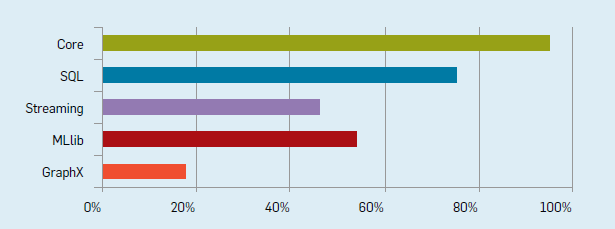
\includegraphics[width=100mm]{./bilder/spark_komponenten_nutzung.png}
  \caption{Nutzung der Komponenten \cite{ZXW+16}}\label{fig:spark_komp_nutzung}
\end{figure}



\noindent
Während Spark Core die Kern-Komponente bildet und alle notwendigen Bausteine für das Framework mitbringt sind die anderen Module auf dem Spark Core Module aufbauen und befassen sich mit spezielleren Bereichen wie SQL, Streaming, maschinelles Lernen oder Graphenberechnungen. In \autoref{fig:spark_core} ist noch einmal eine Übersicht der Komponenten. \\
\noindent
Die Module werden in den folgenden Kapitel von \ref{sec_sparkcore} bis \ref{sec_sparkmlib} näher beleuchtet. \\

\noindent
Dar\"uber hinaus wird in Kapitel \ref{sec_sparkr} SparkR vorgestellt. Das Module gehört nicht direkt, jedoch bietet es interessante Möglichkeiten Datenanylsen mit R zu optimieren bzw. zu beschleunigen.

%Die Aufteilung in die verschiedenen Module macht es sehr gut möglich nur einen Teil der Module zu verwenden. 

\begin{figure}[h]
  \centering
  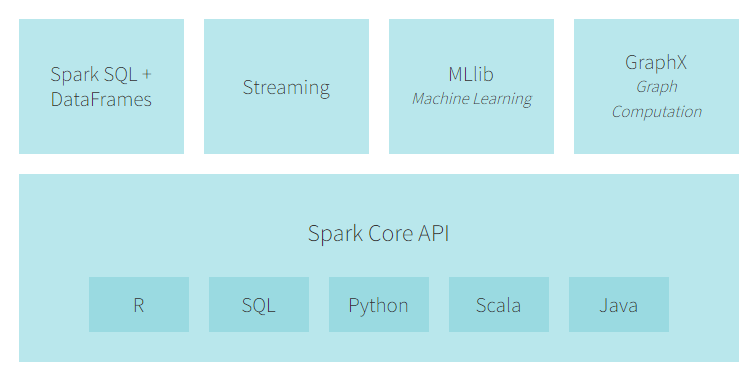
\includegraphics[width=\textwidth]{./bilder/spark_core.png}
  \caption{Spark Core}\label{fig:spark_core}
\end{figure}









\newpage
\subsection{Grundlage des Systems (Spark-Core \& RDD’s)}\label{sec_sparkcore}
%der grundlegende Auführungs-Engine 
Spark Core ist Grundlage der Spark Plattform. Alle anderen Komponenten bauen auf diesen Kern auf. Alle grundlegenden infrastrukturellen Funktionen sind darin enthalten. Darunter zählen diue Aufgabenverwaltung, das Scheduling sowie I/O Funktionen.
Der Kern liefert zum Beispiel die Möglichkeit der Berechnungen direkt im Arbeitsspeicher. 
Das grundlegende Programmiermodell wie das Arbeiten mit den RDD's und die API's für die verschiedenen Sprachen (Java, Scala und Python).  \footnote{Vgl. \cite{DATABRICK_ABOUT}} \\
In der \autoref{fig:spark_core} sind die einzelnen Bausteine innerhalb der Spark Core Komponenten / API zu sehen. 
 


\noindent
Die parallele Verarbeitung wird über den Spark Context realisiert. Der Spark Context wird im eigentlich Programm erzeugt und ist in der Regel dann mit einem Cluster Manager verbunden. Dieser wiederum kennst alle Worker Nodes, die dann die eigentlichen Aufgaben ausführen. Die \autoref{fig:spark_cluster} zeigt wie Spark Context, Cluster Manager und die Worker Nodes zusammen agieren. Damit die Aufgaben über viele Nodes verteilt werden können wird eine Datenstruktur benötigt, die dafür ausgelegt sind. \footnote{Vgl. \cite[101]{BDS16}}

\begin{figure}[h]
  \centering
  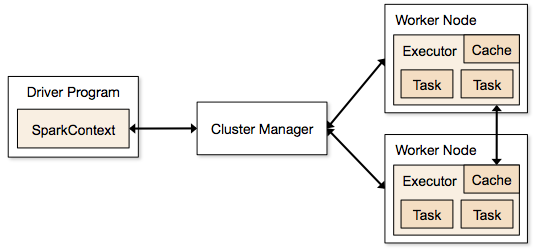
\includegraphics[width=\textwidth,height=50mm]{./bilder/cluster-overview.png}
  \caption{Spark Cluster aus \cite{SPCLUSTER}}\label{fig:spark_cluster}
\end{figure}



\noindent
Die Resilent Distirbuted Datasets (RDD's) zu deutsch elastische, verteilte Datensätze erledigen diese Aufgabe. Es ist die primäre Datenabstraktion in Apache Spark. 
Ein RDD entspricht einer partitionierten Sammlung an Daten. Somit können die Partitionen auf verschiedene Systeme (bzw. Worker) verteilt werden.  \\
Nach der Erstellung sind RDD's nur lesbar. Es ist also nur möglich ein einmal definiertes RDD durch anwendung globaler Operationen in ein neues RDD zu überführen. Die Operationen werden dann auf allen Partitionen des RDD's angewendet. \\
\noindent
Man unterscheidet bei den Operationen zwischen Transformationen (z.B.: filter oder join) und Aktionen (z.B.: reduce, count, collect oder foreach). Transformationen bilden ein RDD auf ein anderes RDD ab. Aktionen bilden ein RDD auf eine andere Domäne ab.\\ %Todo hier nochmal forschen was das bedeutet
\noindent
Eine Folge von Operationen wird Lineage \footnote{RDD Lineage: Logischer Ablaufplan der einzelnen Operationen. Hilft Daten wiederherzustellen falls Fehler aufgetreten sind.} eines RDD's genannt.\footnote{Vgl. \cite{ZC+12}}



\newpage
\subsection{SQL-Abfragen mit (Spark-SQL \& Data Frames)}

Spark-SQL wurde 2014 veröffentlicht. Die Komponente gehört zu den Komponenten aus der Spark-Familie, die am meisten weiterentwickelt werden.
Spark-SQL entstammt dem Apache-Shark. Man wollte die Probleme die es in Apache Shark gab lösen.
\begin{enumerate}
	\item Mit Apache Shark ist es nur möglich auf Daten im Hive\footnote{Apache Hive: Ist eine Erweiterung für Hadoop und ermöglicht Abfragen über SQL zu nutzen.} Katalog zuzugreifen. 
	\item Shark lässt sich nur über selbst geschriebene SQL's aufrufen. 
	\item Hive ist nur für MapReduce optimiert
\end{enumerate}

\noindent
Es werden zwei wesentliche Anwendungsfälle kombiniert. Zum einen ermöglicht es relationale Querys zu schreiben und zum anderen prozedurale Algorithmen einzusetzen. 
Dafür werden neben den RDD's die DataFrames als weitere Datenstruktur eingeführt.\\

\noindent
Die Abfragen werden zuerst in den DataFrame-Objekten gespeichert. Erst nach der Initialisierung werden diese SQL's dann ausgewertet. Für die Auswertung und Optimierung kommt Catalyst\footnote{Catalyst: Ist eine Optimierungsengine für relationale Ausdrücke.} zum Einsatz. Nach der Auswertung werden die Abfragen gegebenenfalls opptimiert und danach in Spark-Optionen auf RDD's übersetzt. In \autoref{fig:spark_sql} sind die Phasen vom SQL-Query bis hin zu den RDD's dargestellt. In den Boxen mit abgerundenten Ecken befinden sich Catalyst-Trees.

\begin{figure}[h]
  \centering
  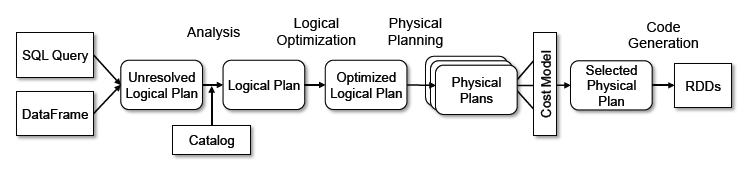
\includegraphics[width=\textwidth]{./bilder/spark_sql.png}
  \caption{Phasen der Query Planung in Spark SQL \cite{AXL+15}}\label{fig:spark_sql}
\end{figure}

\noindent
Mit Spark-SQL hat man erreicht auf relationale Daten zuzugreifen. Es wurde eine hohe Performance aufgrund etablierter DBMS-Techniken erreicht.
Neue Datenquellen lassen sich leicht anschließen und integrieren.
Zusätzliche Erweiterungen wie maschinelles Lernen und Berechnungen von Graphen sind zusätzlich nutzbar.\footnote{Vgl. \cite{AXL+15}} \\

\newpage
\subsection{Verarbeitung von Datenströmen (Spark-Streaming)}

%Hier nochmal nachlesen, das sieht ganz gut aus. https://www.infoq.com/articles/apache-spark-streaming

Die Spark-Streaming Bibliothek ermöglicht das Verarbeiten von Datenströmen. Auch hier dienen die RDD's als Grundlage. Die RDD's werden zu DStreams erweitert. DStreams (discretized streams) sind Objekte, die Informationen enthalten, die in Verbindung mit Zeit stehen. DStreams sind intern eine Sequenz von RDD's und werden aus diesem Grund diskrete Streams genannt.
Auch DStreams haben die bereits aus \ref{sec_sparkcore} bekannten zwei Operationen (Transformation und Aktion). \\

\noindent
Um Datenströme zu empfangen wird ein Empfänger (Receiver) auf einem Worker-Knoten gestartet. Die eingehenden Daten werden in kleinen Datenblöcken gespeichert. Dafür werden die Daten innerhalb eines vorgegebenen Zeitfenster gepuffert. Pro Zeitfenster werden die Daten in dem Puffer in eine Partition eines RDD abgelegt.\footnote{Vgl. \cite{BDS16}} \\

\noindent
In der Spark-Streaming Bilbliothek sind bereits einige Empfänger wie Kafka\footnote{Apache Kafka dient zur Verarbeitung von Datenströmen dient.}, Twitter\footnote{Twitter: ist ein Mikrobloggingdinst. Nutzer können über das Portal Kurznachrichten verbreiten. } oder TCP-Sockets\footnote{TCP-Sockets: Sind Kommunkationsendpunkte, die zur Netzwerkkommunikation genutzt werden. } enthalten. \\
\autoref{fig:spark_streaming} zeigt den Ablauf vom Eingang der Daten über die Verarbeitung bis hin zur Ausgabe auf zum Beispiel Dashboard oder der Speicherung in Datenbankbanken.

\begin{figure}[h]
  \centering
  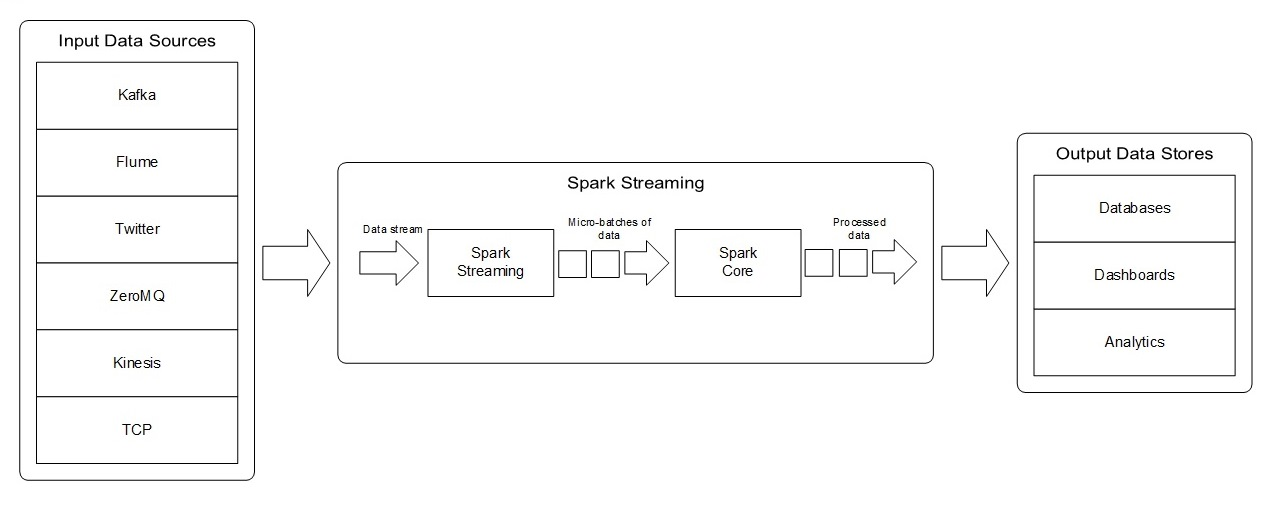
\includegraphics[width=\textwidth]{./bilder/spark_streaming.jpg}
  \caption{Spark Streaming Ablauf \cite{INFOQ_STREAMING}}\label{fig:spark_streaming}
\end{figure}





\newpage
\subsection{Berechnungen auf Graphen (GraphX)}

Das GraphX Framework ermöglicht die Berechnungen auf Graphen. Die Grundlage sind auch hier die RDD's. Also Graphenstrukturen werden Property-Graphen genutzt. 
Property-Graphen sind gerichtete Multigraphen. Das heißt der Grpah besteht aus Ecken(Konten) und Kanten. An den Kanten können Eigenschaften hinterlegt sein.\\

\noindent
In dem GraphX Framework werden diese Graphen aus Tupeln aus RDDs gebildet. In dem ersten RDD sind die Ecken und in dem zweiten die Kanten enthalten. Um die Graphen auf mehrere Maschinen zu verteilen werden diese entlang der Kante geteilt. Man spricht hier vom sogenannten Edge Cut Verfahren. Eine einzelne Ecke kann somit auf mehreren Maschinen existieren. Um Änderungen an einer Ecke über alle Kopien auf den Maschinen zu propagieren wird zusätzlich eine Routing-Tabelle gepflegt. Über diese sind alle Kopien von Ecken bekannt und bei Änderungen einer Ecke werden alle Maschinen entsprechend informiert. 
In der folgenden \autoref{fig:spark_graphx} ist ein verteilter Property-Graph abgebildet. Zusätzlich sind die verschiedenen RDD's für Knoten(Vertex), Kanten(Edge) und die Routing-Tabelle abgebildet.

\begin{figure}[h]
  \centering
  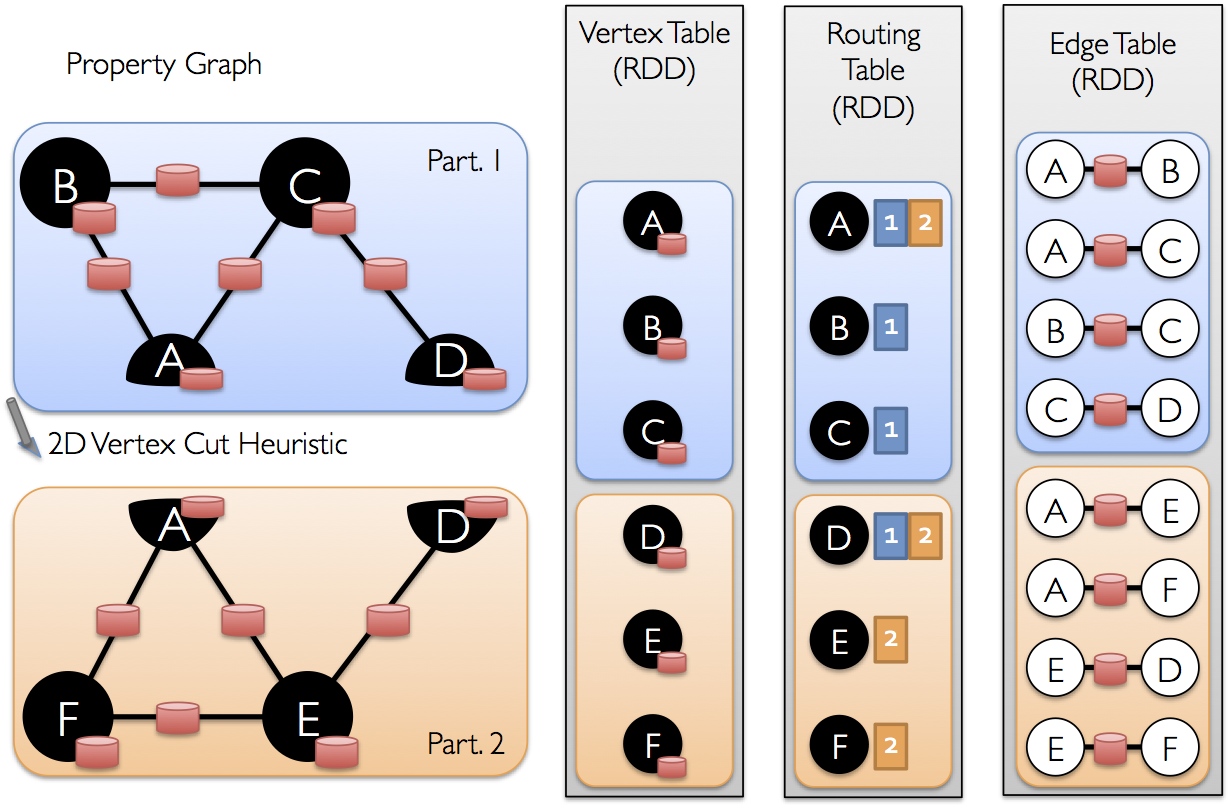
\includegraphics[width=100mm]{./bilder/vertex_routing_edge_tables.png}
  \caption{Property-Graph mit den dezugehörigen RDD's \cite{SPGRAPHX}}\label{fig:spark_graphx}
\end{figure}





\newpage
\subsection{Maschinelles Lernen (MLlib)}\label{sec_sparkmlib}



\newpage
\subsection{Skalierung von R Programmen (SparkR)}\label{sec_sparkr}



\newpage
\section{Mehrere Komponenten im Verbund}

\newpage
\section{Performance}
%PAPER: Scaling Spark in the Real World
Analysen von Performance Probleme erweisen sich mitunter als sehr schwierig. Apache Spark bringt zwar die seiteneffektfreie API mit, jedoch kann trotzdem eine Menge schief gehen. Für Entwickler ist es immer schwer im Hinterkopf zu behalten, dass Operationen auf vielen verteilten Rechnern ablaufen. \\ \\
Über eine Webbasierte Übersicht, die in \autoref{fig:spark_ui_worker} zu sehen ist,ist es Möglich Informationen zu dann aktuell laufenden Auswertungen und Dauer von Ergebnissen etc. zu bekommen. \footnote{Vgl. \cite[12]{AAWS15}}

\begin{figure}[h]
  \centering
  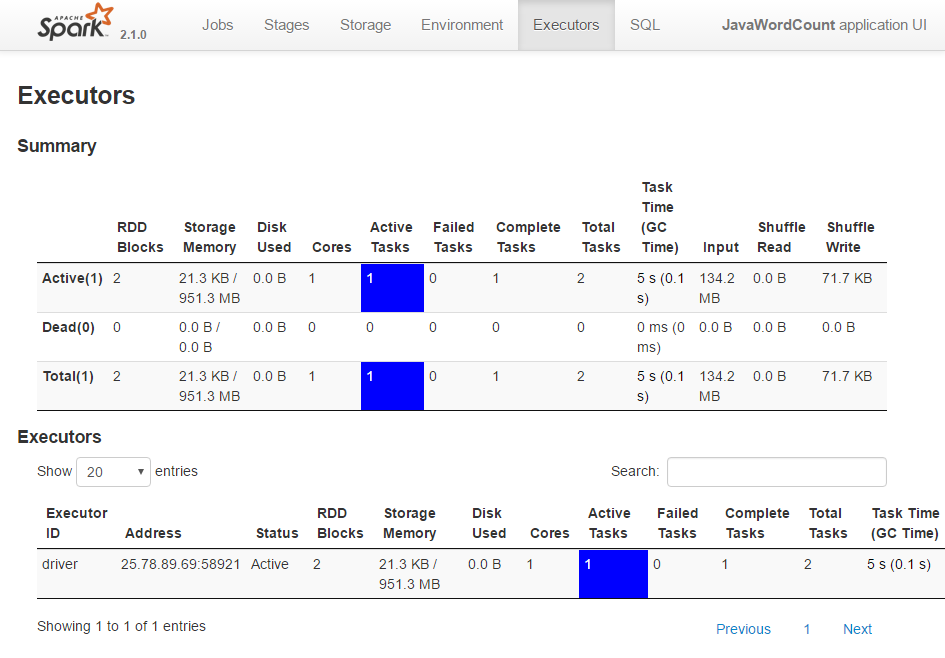
\includegraphics[width=\textwidth]{./bilder/spark_ui_worker.PNG}
  \caption{Spark Web UI: Zusammenfassung der Worker}\label{fig:spark_ui_worker}
\end{figure}

%eventuell in die Performance section
\noindent
Speziell beim Thema SQL-Abfragen ist es enorm wichtig sich für die richtigen Anweisungen zu entscheiden um keine langsamen Operationen zu haben. 
Hier gibt es sehr große Geschwindigkeitsunterschiede.



\subsection{Besonderheiten bei der Speichernutzung}
Die Wahl einer geeigneten bzw. speichereffizienten Datenstruktur wir oftmals unterschätzt. 
Spark geht davon aus, eine Datei in Blöck einer bestimmten Größe geladen wird. In der Regel 128MB. Zu beachten ist jedoch, dass beim dekomprimieren größere Blöcke entstehen können. So können aus 128MB schnell 3-4GB große Blöcke in dekompriemierten Zustand werden. \\ 

\noindent
Um das Speichermanagement zu verbessern wurde ein per-node allocator implementiert. Dieser verwaltet den Speicher auf einer Node. 
Der Speicher wir in drei Bereiche geteilt. 
Speicher zum verarbeiten der Daten.  
Speicher für die hash-tables bei Joins oder Aggretaions
Speicher für \"unrolling\" Blöcke, um zu prüfen ob die einzulesenden Blöcke nach dem entpacken immer noch klein genug sind damit diese gecached werden können.
Damit läuft das System robust über für Anwendungsbereiche mit sehr vielen Nodes sowie mit ganz wenigen.\footnote{Vgl. \cite{ADD+15}}

\subsection{Netzwerk und I/O-Traffic}

Mit Apache Spark wurden schon Operationen bei denen über 8000 Nodes involviert waren und über 1PB an Daten verarbeitet wurden durchgeführt.
Das beansprucht natürlich die I/O Schicht enorm. 


Um I/O Probleme zu vermeiden, bzw. diese besser in den Griff zu bekommen wurde als Basis das Netty-Framework\footnote{Netty: High-Performance Netzwerk Framework} verwendet.
\begin{itemize}
	\item Zero-copy I/O:\\
	Daten werden direkt von der Festplatte zu dem Socket kopiert. Das vermeidet Last an der CPU bei Kontextwechseln und entlastet zusätzlich den JVM\footnote{JVM: Todo} garbage collector\footnote{garbage collector: Todo}
	\item Off-heap network buffer management:\\
	Netty verwaltet einige Speichertabellen außerhalb des Java Heap Speichers um Probleme mit den JVS garbage collector zu vermeiden.
	\item Mehrfache Verbindungen:\\
	Jeder Spark worker kann mehrere Verbindungen parallel bearbeiten.
\end{itemize}


%\newpage
\section{Nutzung \& Verbreitung}

Durch die Unterstützung der drei Programmiersprachen skala, pathon und java ist die Arbeit mit Apache Spark einfacher, als wenn es nur einen einzige exotische Programmiersprache zur Nutzung gäbe. \\

\noindent
Apache Spark unterstützt zudem noch verschiedene Datenquellen und Dateiformate.  Zu den Datenquellen zählen die das Dateisystem S3\footnote{S3 (Simple Storage Service): ist ein Filehosting-Dienst von Amazon der beliebig große Datenmengen speichern kann} von Amazon und das HDFS\footnote{HDFS (Hadoop Distributed File System): Ist ein hochverfügbares Dateisystem zu Speicherung sehr großer Datenmengen}.
Die Dateiformate können strukturiert (z.B.: CSV, Object Files), semi-strukturiert (z.B.: JSON) und unstrukturiert (z.B.: Textdatei) sein.\\

\noindent
Unter den Mitwirkenden(Contributors) zählen über 400 Entwickler aus über 100 Unternehmen, Stand 2014.\\
Es gibt über 500 produktive Installationen. \cite{ADD+15} \\ %PAPER: Scaling Spark in the Real World\\

\noindent
%http://spark.apache.org/community.html
Seit einigen Jahren finden weltweit jährlich unter dem Namen Spark Summit Konferenzen statt. \cite{SPCOM}\\



%DONE: https://www.heise.de/developer/meldung/Big-Data-Umfrage-zur-Verbreitung-zu-Apache-Spark-2529126.html
\noindent
Heise.de beauftrage 2015 eine Umfrage in der 2136 Teilnehmer befragt wurden \cite{HEISEBIGDATA}. Diese gaben an, dass 31\% Prozent den Einsatz derzeit prüfen. 13\% Nutzen bereits Apache Spark und 20\% planten den Einsatz noch in dem damaligen Jahr.
Scala lag als Programmiersprache mit großen Abstand vorn. Die Nutzung innerhalb verschiedener Berufsgruppen war sehr ähnlich. Mit 16\%  lag bei den Telekommunikationsunternehmen der Einsatz am höchsten. Eine detaillierte Übersicht ist in \autoref{fig:nutzung} zu sehen.
\begin{figure}[h]
  \centering
  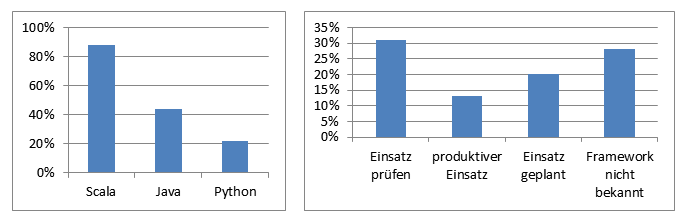
\includegraphics[width=\textwidth]{./excel/Nutzung.png}
  \caption{Einsatz \& Verbreitung}\label{fig:nutzung}
\end{figure}


